\chapter{Anhang}
\label{appendix}

\section{Evaluationsparameter}
\label{sec:eval_param}



\sisetup{round-mode = places, round-precision = 2, scientific-notation = fixed, fixed-exponent = 0}
\begin{table}[!htbp]
    \centering
    \begin{tabular}{crSSSS}
        \hline
        & Anzahl an Samplen \(n\)& \( 1000\)\\
        & {Diskretisierung Schrittweite \gls{symb:h}} & \(0.2 \mathrm{s}\)\\
        & Planungshorizont \(t_\mathrm{planhozion}\)& \(15 \mathrm{s}\)\\
        & Nauplanungsintervall \gls{symb:t_verarb} & \(1\mathrm{s}\) \\
        & Fahrstreifenwechseldauer \gls{symb:t_lcd} & \(4\mathrm{s}\) \\
        & Gew\"unschter Zeitsabstand \gls{symb:t_abs} & \(1.8\mathrm{s}\) \\
        & Grenzverz\"ogerung \gls{symb:b_krit} & \(1.5\mathrm{m/s^2}\) \\   
        & Angenommen Beschleunigung nach Kooperation \gls{symb:a_lcend} & \(0.5\mathrm{m/s^2}\) \\           
         \hline
    \end{tabular}
    \caption[Simulations Parameter]{Simulations Parameter
    }\label{tab:Simpara}
\end{table}


\sisetup{round-mode = places, round-precision = 2, scientific-notation = fixed, fixed-exponent = 0}
\begin{table}[!htbp]
    \centering
    \begin{tabular}{crSSSS}
        \hline
        & & \(a\)  [m/s\textasciicircum 2] & \( v\) [km/h] & \(d_{normal}\) [m] \\%
        \hline
         & \gls{symb:f_opt} & 00.00e+00 & 48.00e+00 & 1.1e+00\\
         & \gls{symb:f_discstartp} & 1.50e+00 & 58.00e+00 & x \\
         & \gls{symb:f_discstartn} & -1.50e+00 & 33.00e+00 & 1.00e+00\\
         & \gls{symb:f_infstartp} & 5.00e+00 & x & x \\
         & \gls{symb:f_infstartn} & -7.50e+00 & 0.00e+00 & 0.1e+00\\
          \hline
    \end{tabular}
    \caption[Grenzwerte des Kostenfunktionals]{Grenzwerte des Kostenfunktionals. \gls{symb:f_opt} legt den Optimalwert fest. \gls{symb:f_discstartp} und \gls{symb:f_discstartn} den Beginn der Diskomfortzonen und \gls{symb:f_infstartp} und \gls{symb:f_infstartn} den Beginn der Unrealisierbarkeitszone
    }\label{tab:Kostfunc}
\end{table}



\sisetup{round-mode = places, round-precision = 2, scientific-notation = fixed, fixed-exponent = 0}
\begin{table}[!htbp]
    \centering
    \begin{tabular}{crSSSS}
        \hline
        & Wunschgeschwindigkeit \( v_{0} \) & \( 48  \mathrm{\frac{km}{h}}\)\\
        & Minimalabstand \(s_{0}\) & \(2\mathrm{m}\)\\
        & Gew\"unschte Zeitl\"ucke \( T \) & \(1.5\mathrm{s}\) \\
        & Maximale Beschleunigung \( a \) & \(2\mathrm{\frac{m}{s^2}}\) \\
        & Komfortable Verz\"ogerung \( b \) & \(2\mathrm{\frac{m}{s^2}}\) \\
        & Beschleunigungsexponent \( \delta \) & \(4\)\\
        
         \hline
    \end{tabular}
    \caption[IDM Parameter]{\gls{idm} Parameter
    }\label{tab:IDMpara}
\end{table}


\section{Bildabfolgen}
\label{sec:bildabfolge}

\begin{figure}[!htbp]
    \centering
    \label{fig:abfolgecoop}
    \subfigure[t = 1s ]{
        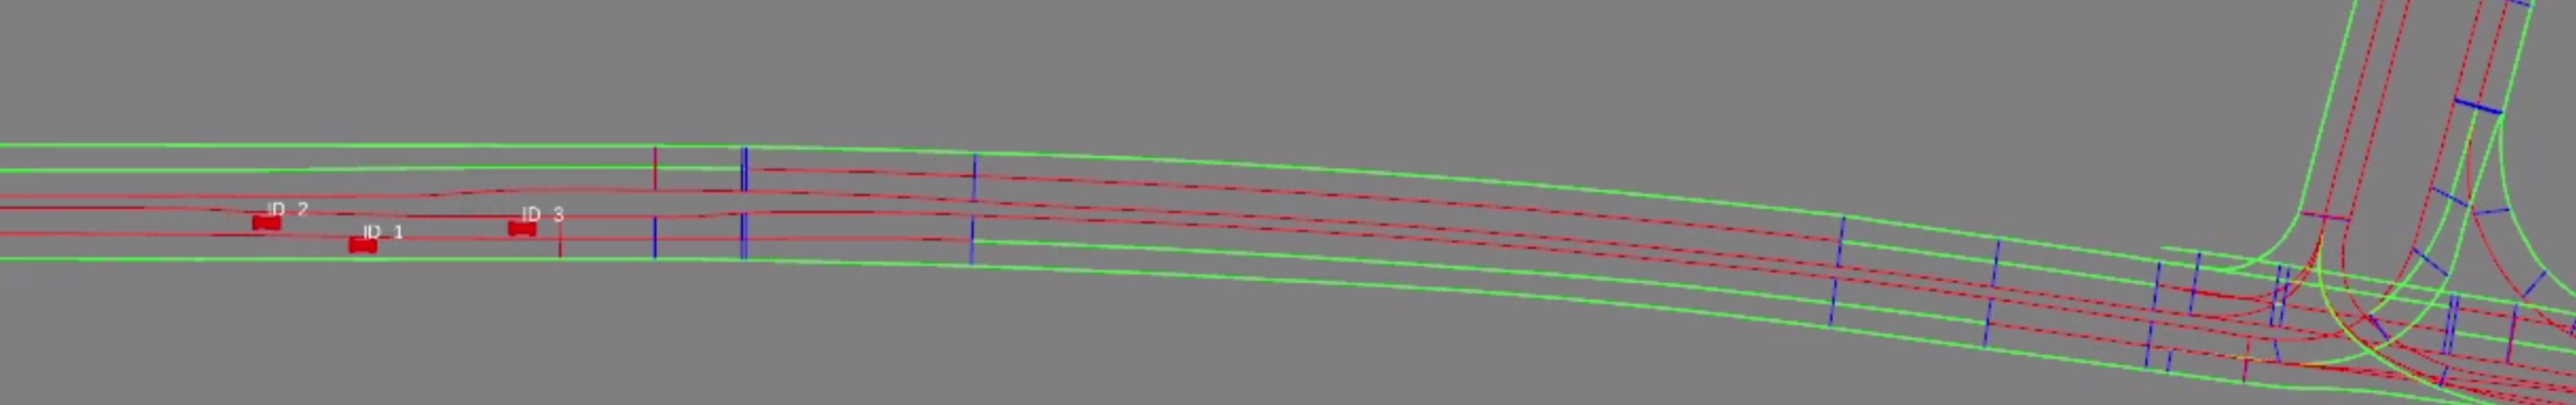
\includegraphics[width =  0.9 \textwidth]{coopt_1.pdf}
    }
    \subfigure[t = 3s ]{
        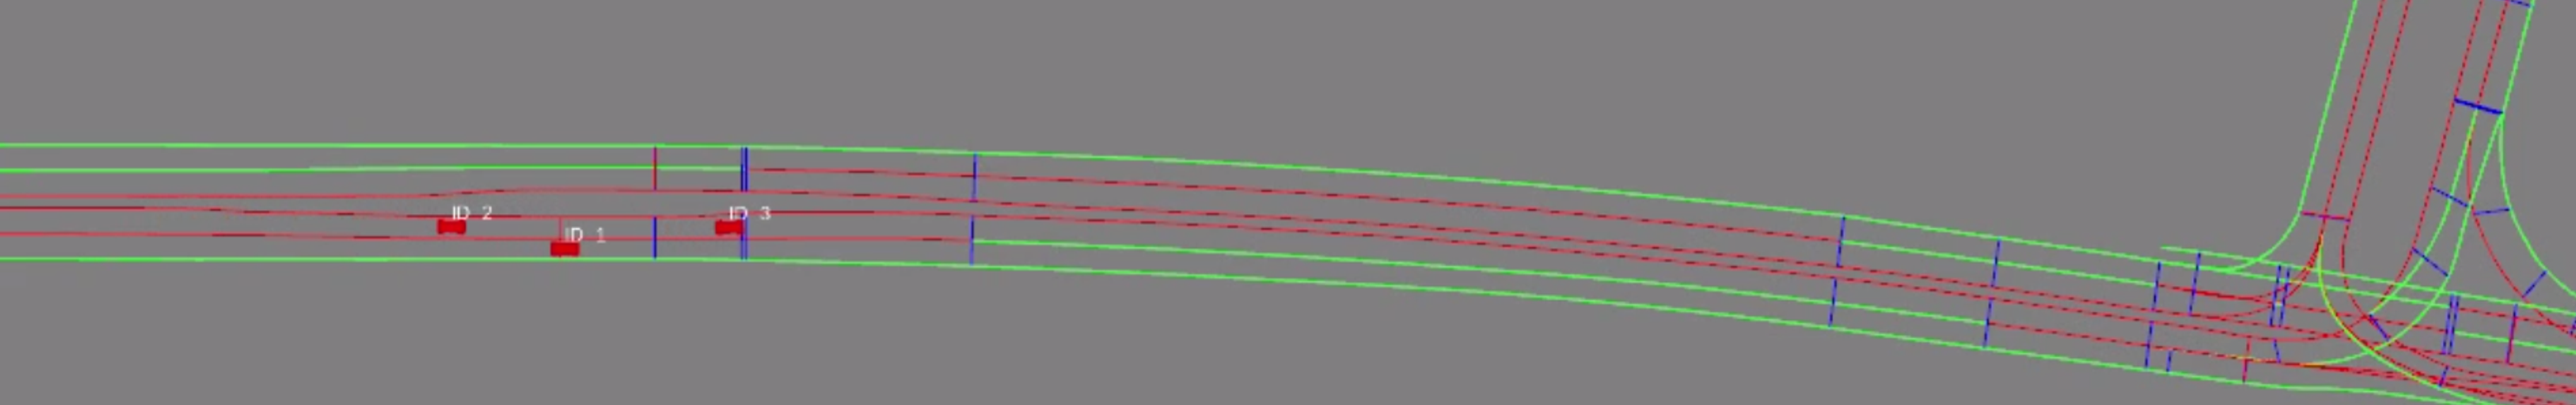
\includegraphics[width =  0.9 \textwidth]{coopt_3.pdf}
    }
    \subfigure[t = 5s ]{
        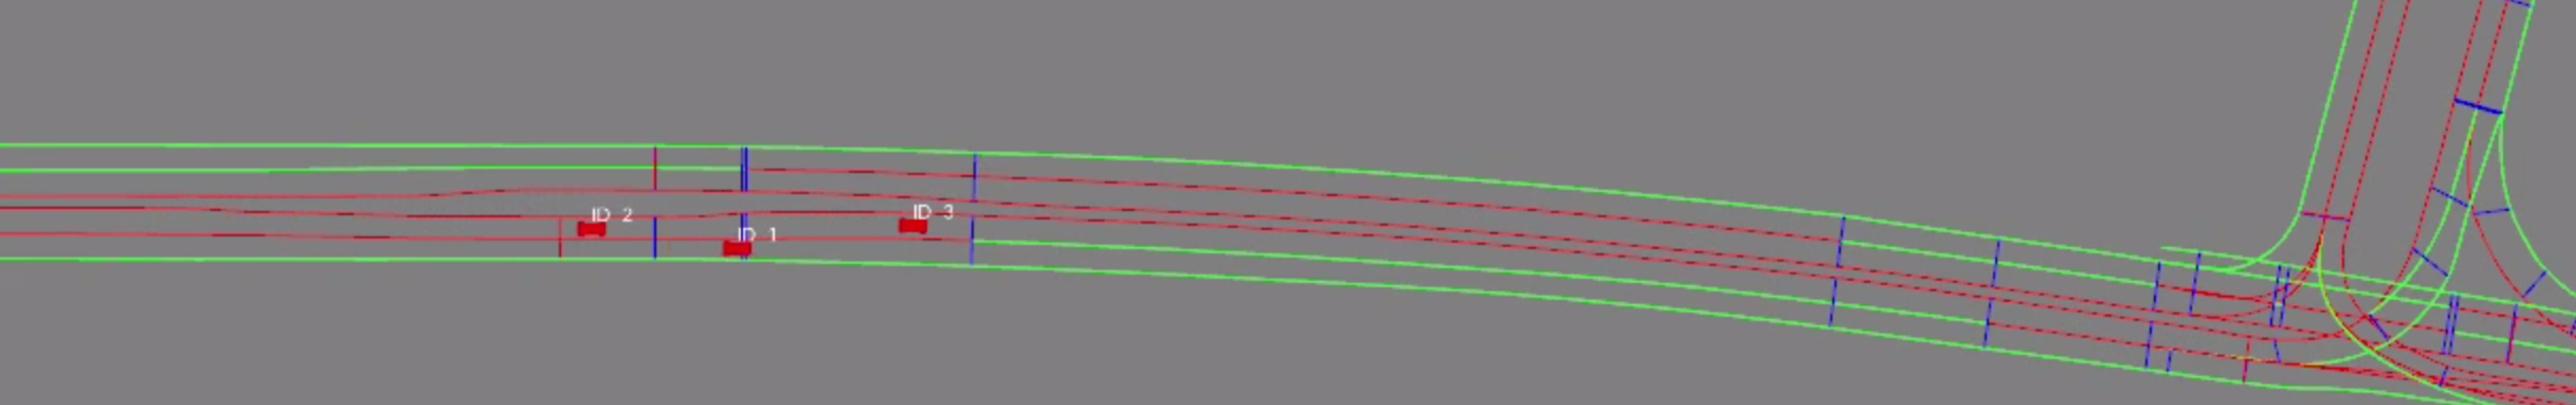
\includegraphics[width =  0.9 \textwidth]{coopt_5.pdf}
    }
    \subfigure[t = 7s ]{
        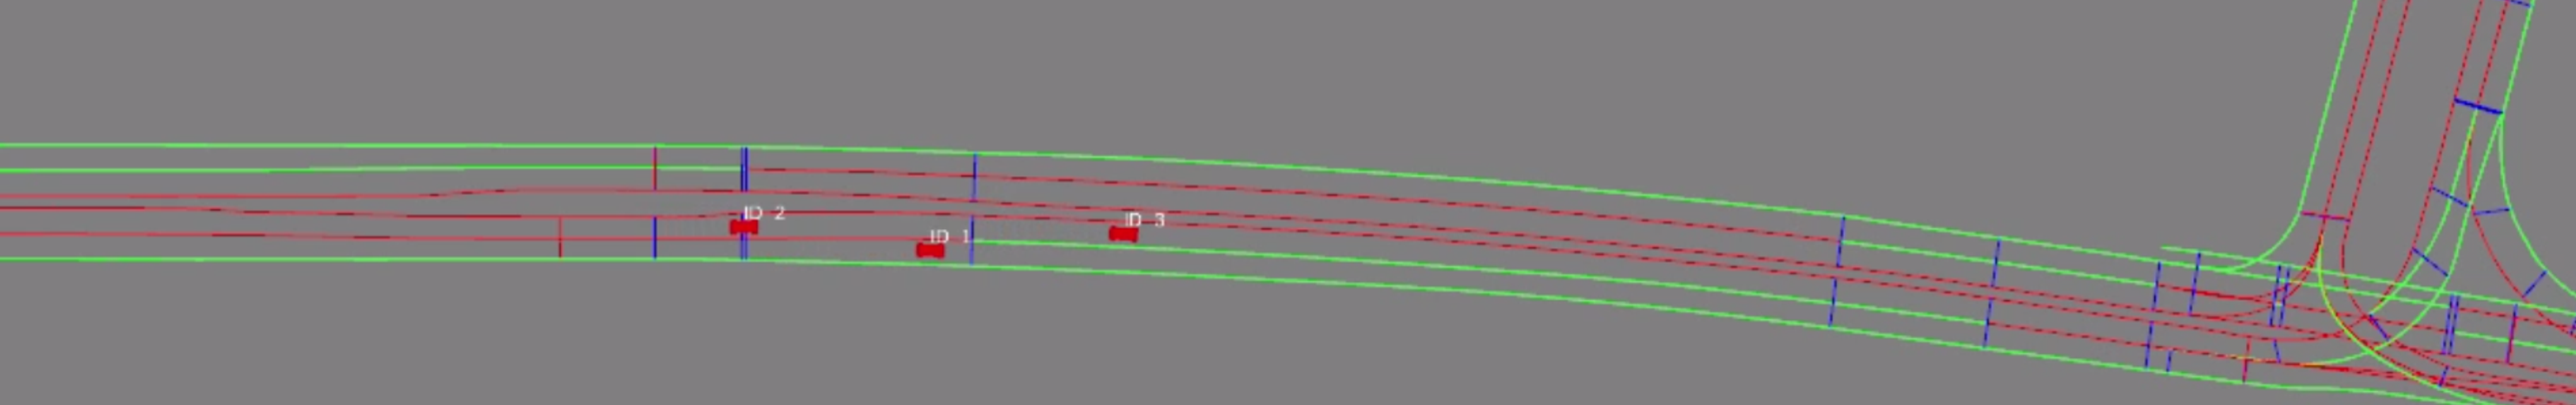
\includegraphics[width =  0.9 \textwidth]{coopt_7.pdf}
    }
    \subfigure[t = 9s ]{
        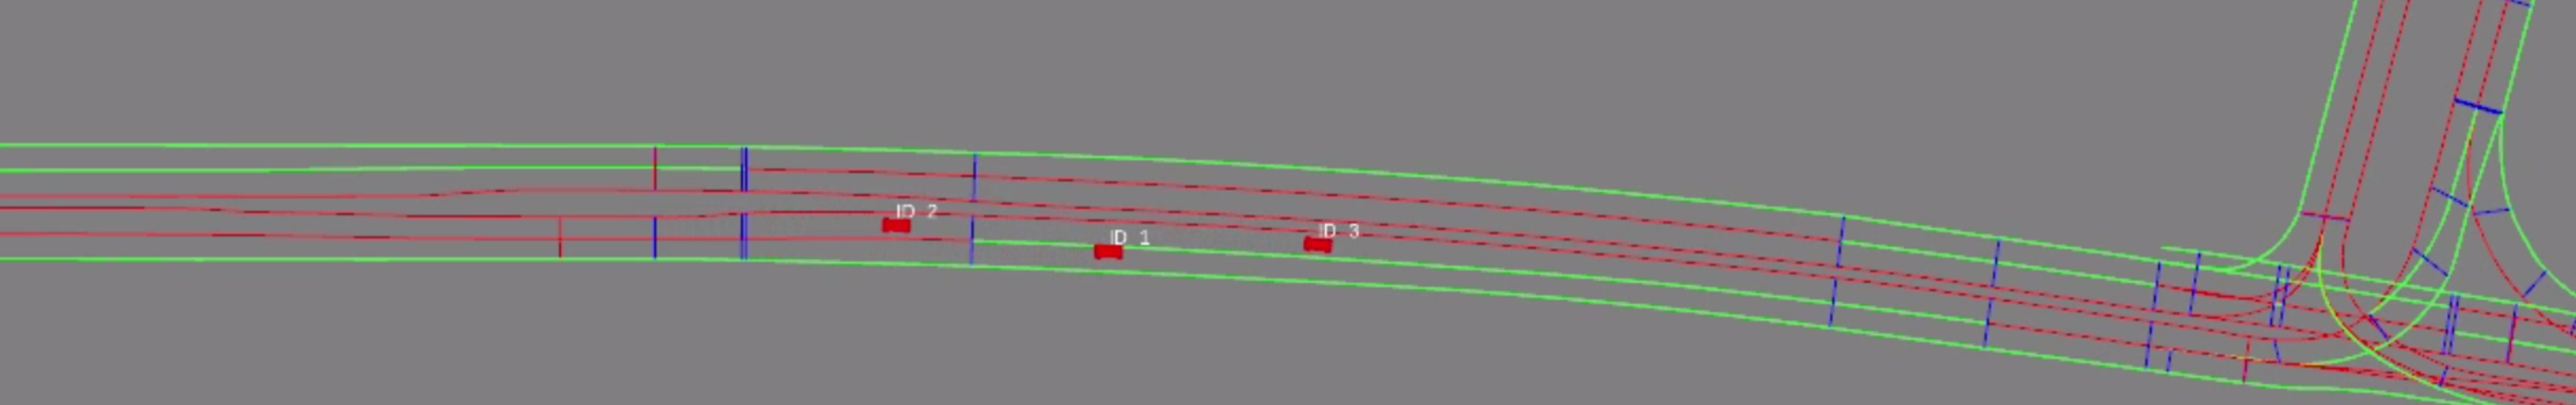
\includegraphics[width =  0.9 \textwidth]{coopt_9.pdf}
    }
    \subfigure[t = 11s ]{
        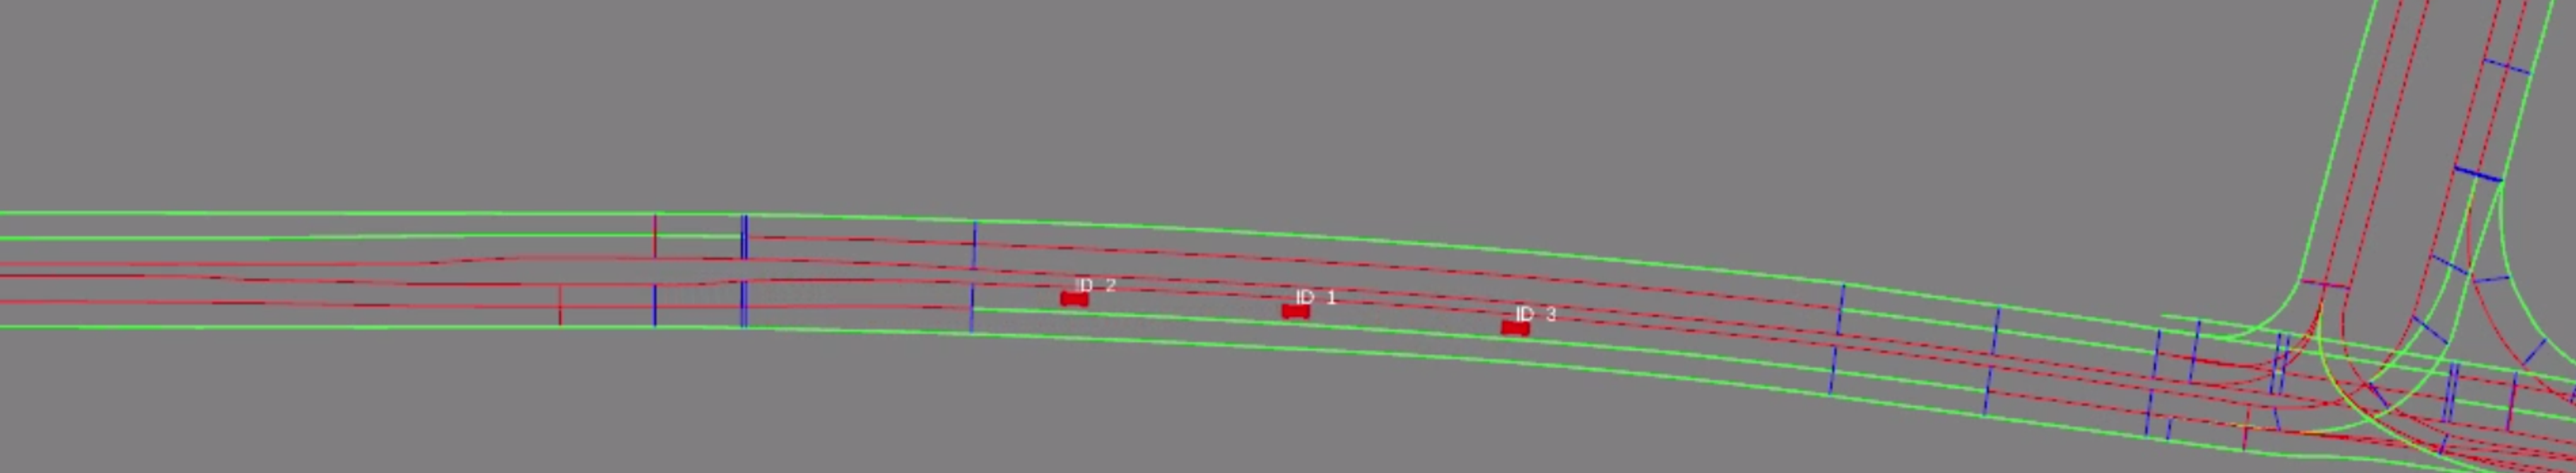
\includegraphics[width =  0.9 \textwidth]{coopt_11.pdf}
    }
    \subfigure[t = 13s ]{
        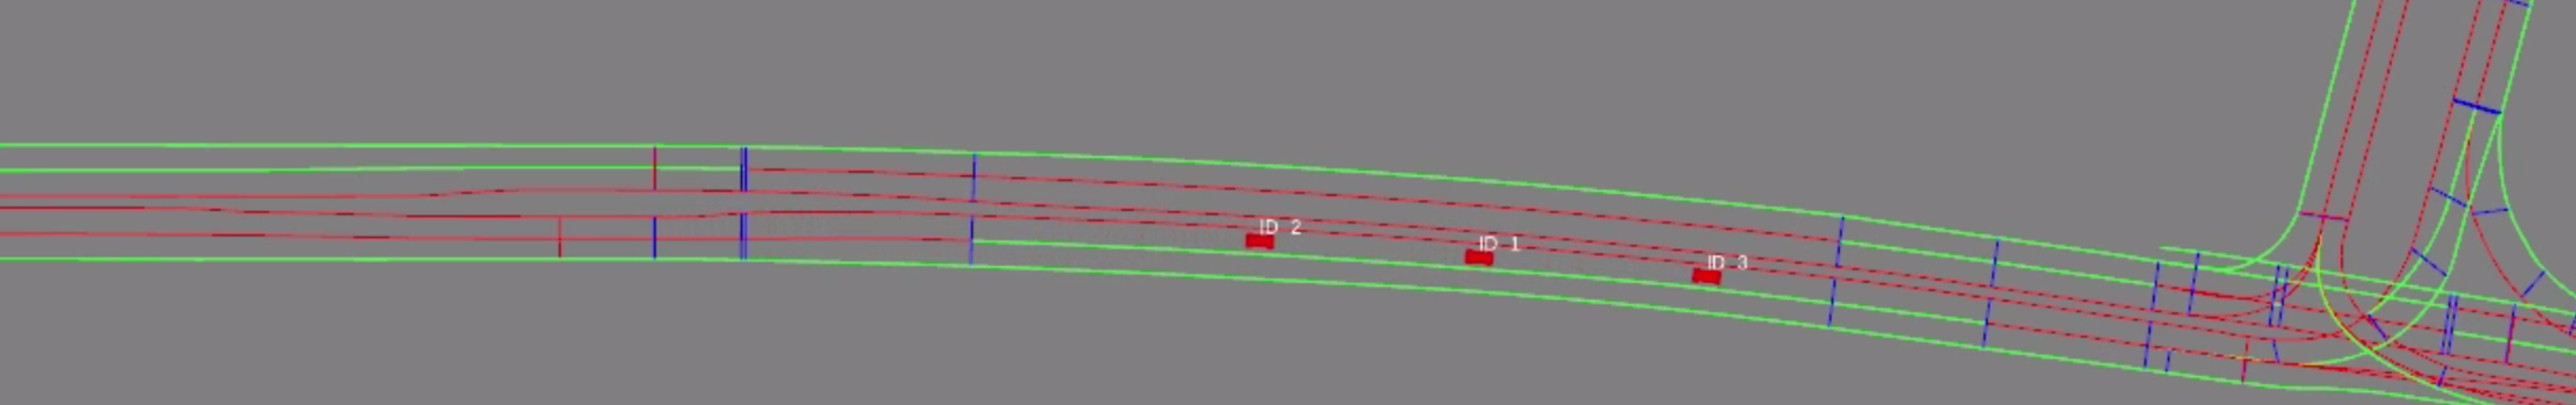
\includegraphics[width =  0.9 \textwidth]{coopt_13.pdf}
    }
    \caption[Bildabfolge kooperativ]{Bildabfolge eines kooperativen Fahrstreifenwechsels bei sek\"undlicher Neuplanung}
\end{figure}


\begin{figure}[!htbp]
    \centering
    \label{fig:abfolgeego}
    \subfigure[t = 1s ]{
        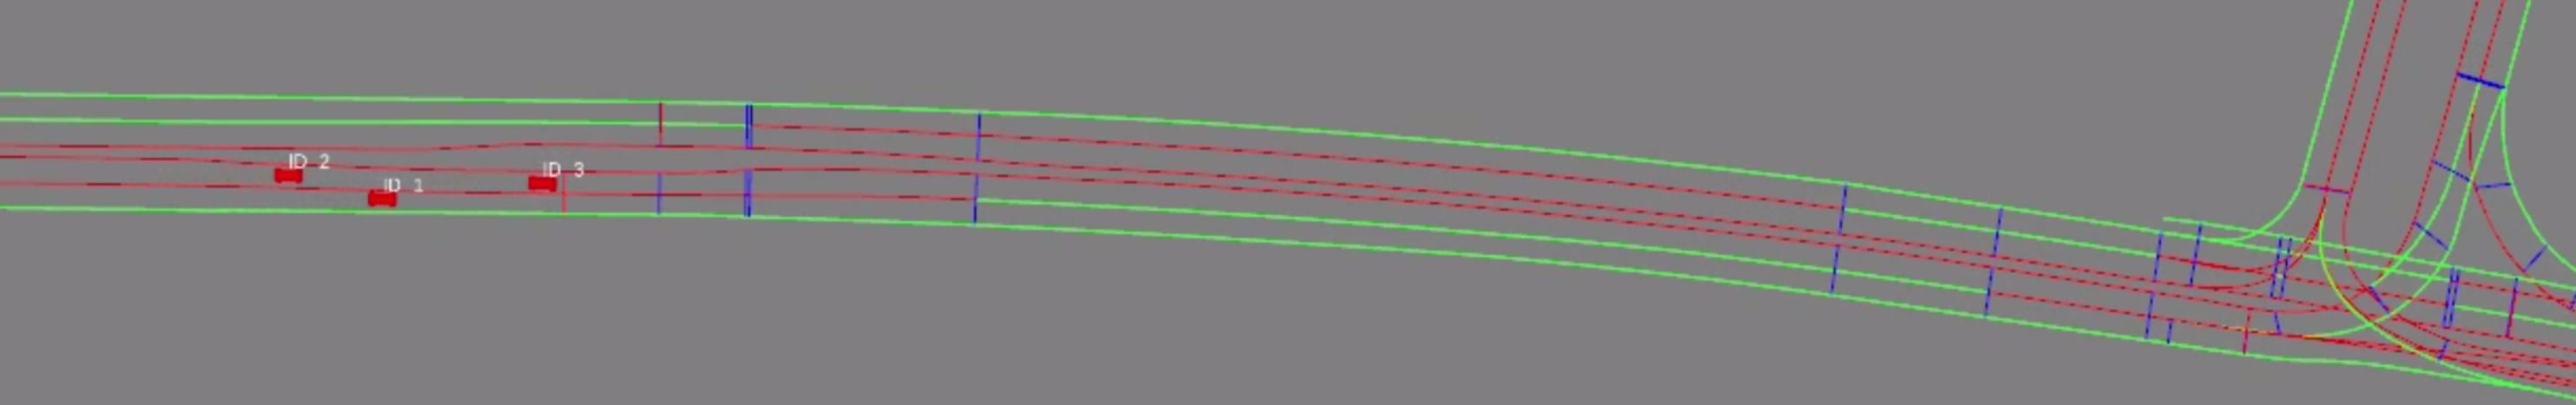
\includegraphics[width =  0.9 \textwidth]{egot_1.pdf}
    }
    \subfigure[t = 3s ]{
        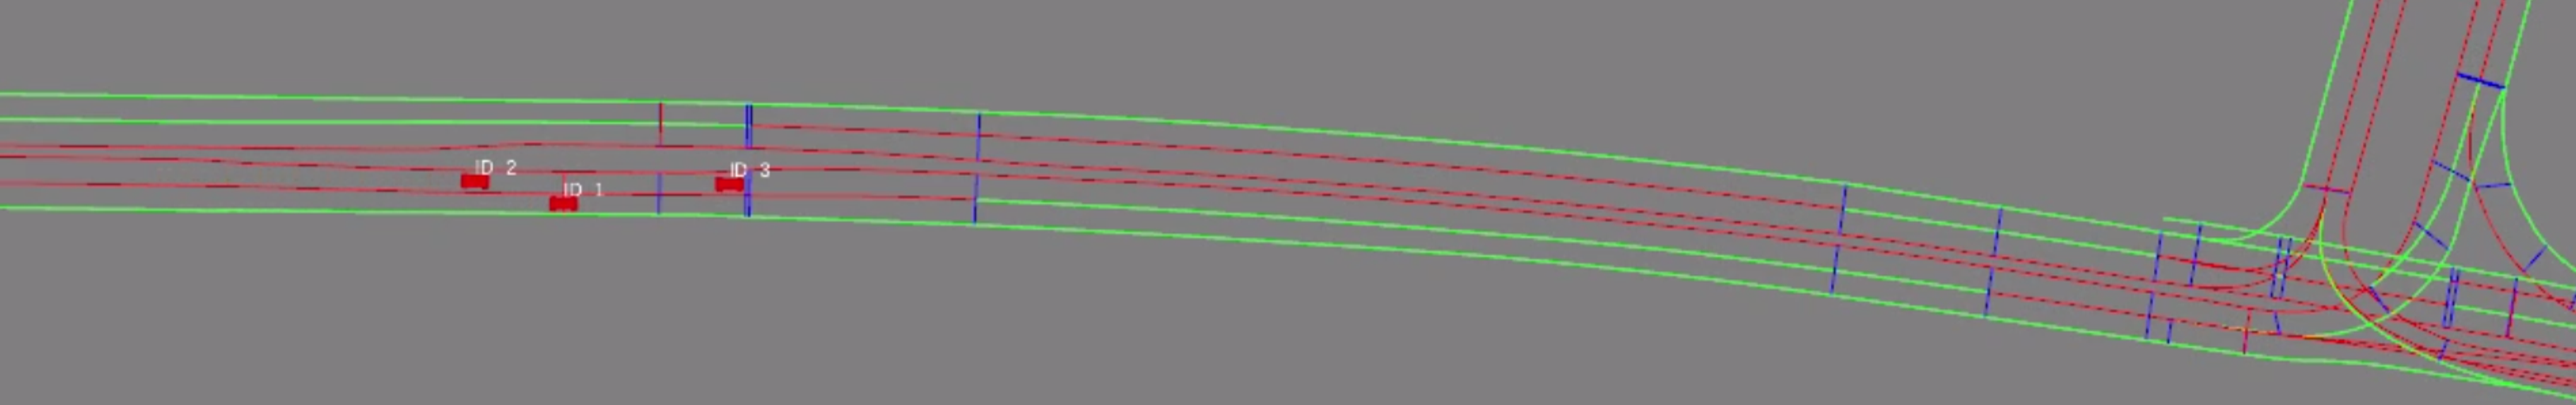
\includegraphics[width =  0.9 \textwidth]{egot_3.pdf}
    }
    \subfigure[t = 5s ]{
        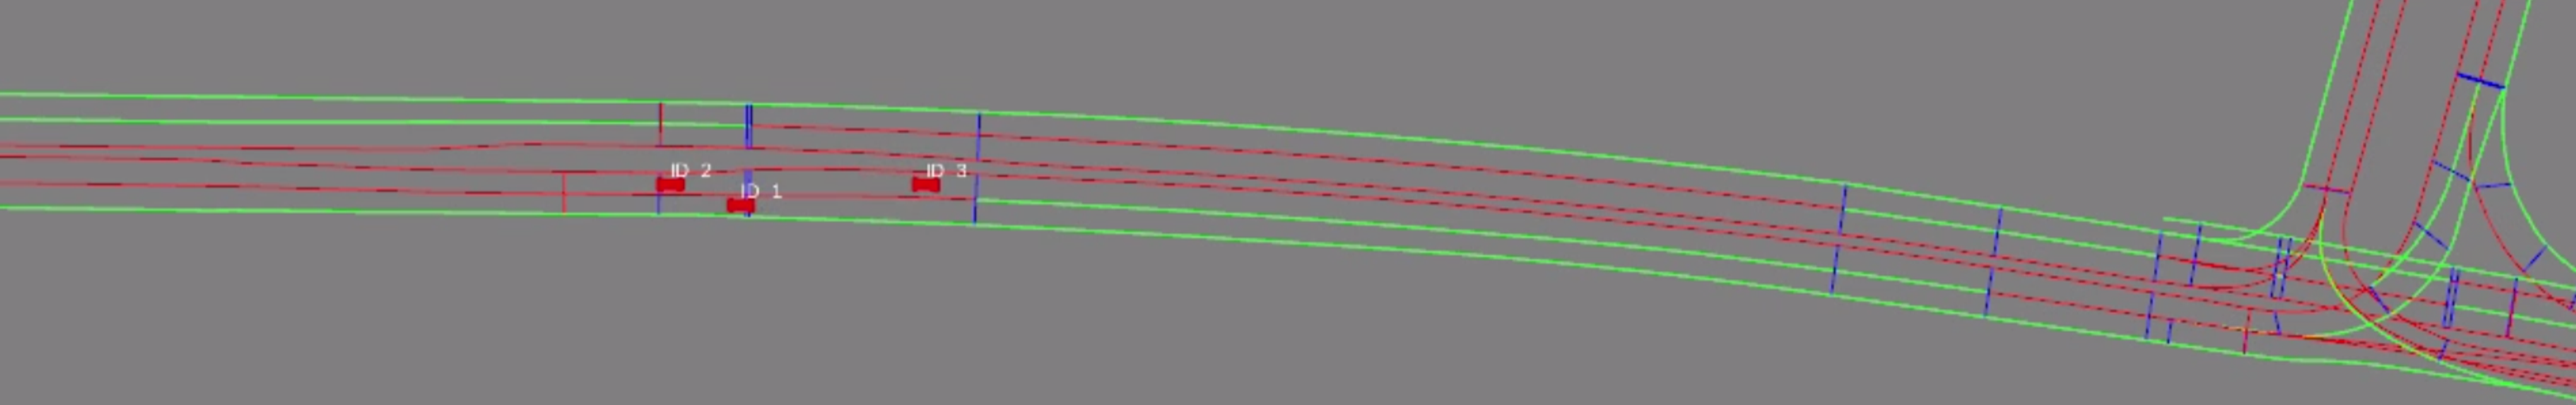
\includegraphics[width =  0.9 \textwidth]{egot_5.pdf}
    }
    \subfigure[t = 7s ]{
        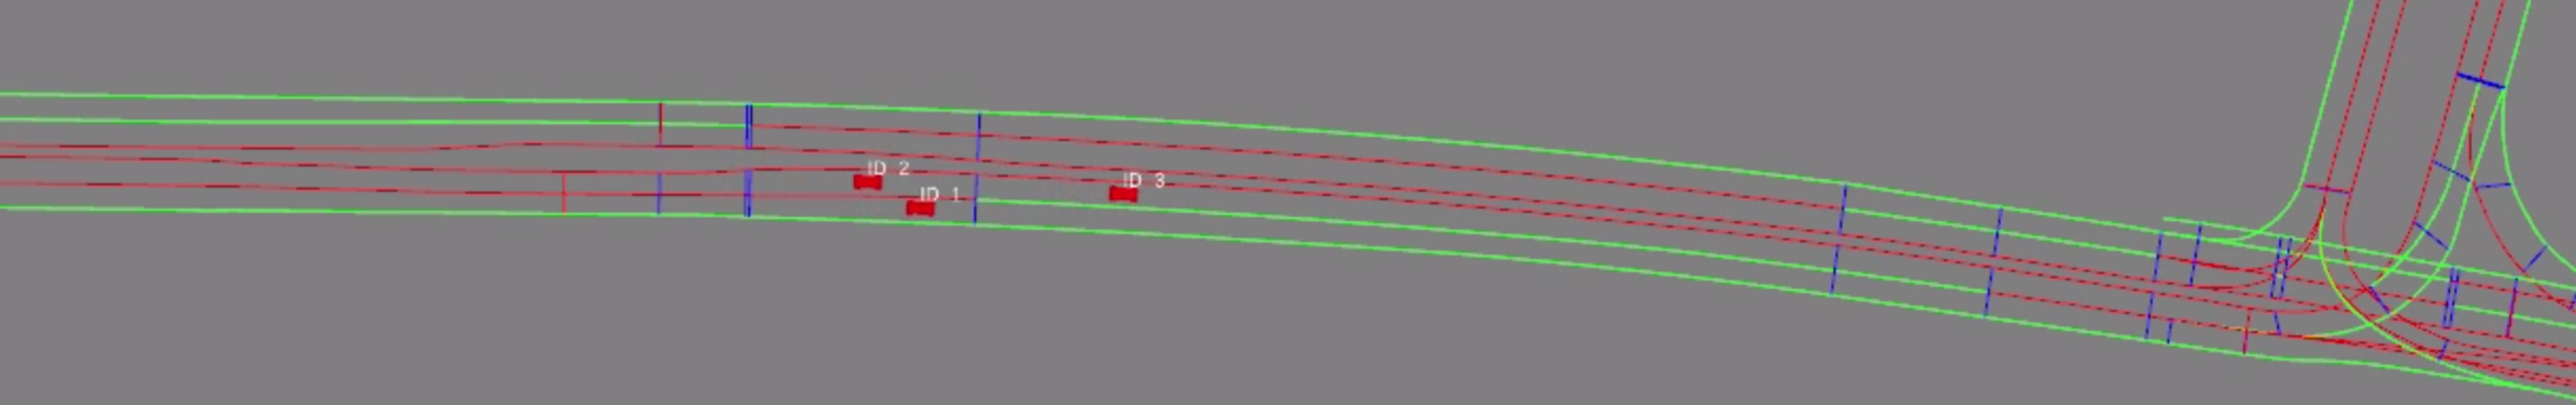
\includegraphics[width =  0.9 \textwidth]{egot_7.pdf}
    }
    \subfigure[t = 9s ]{
        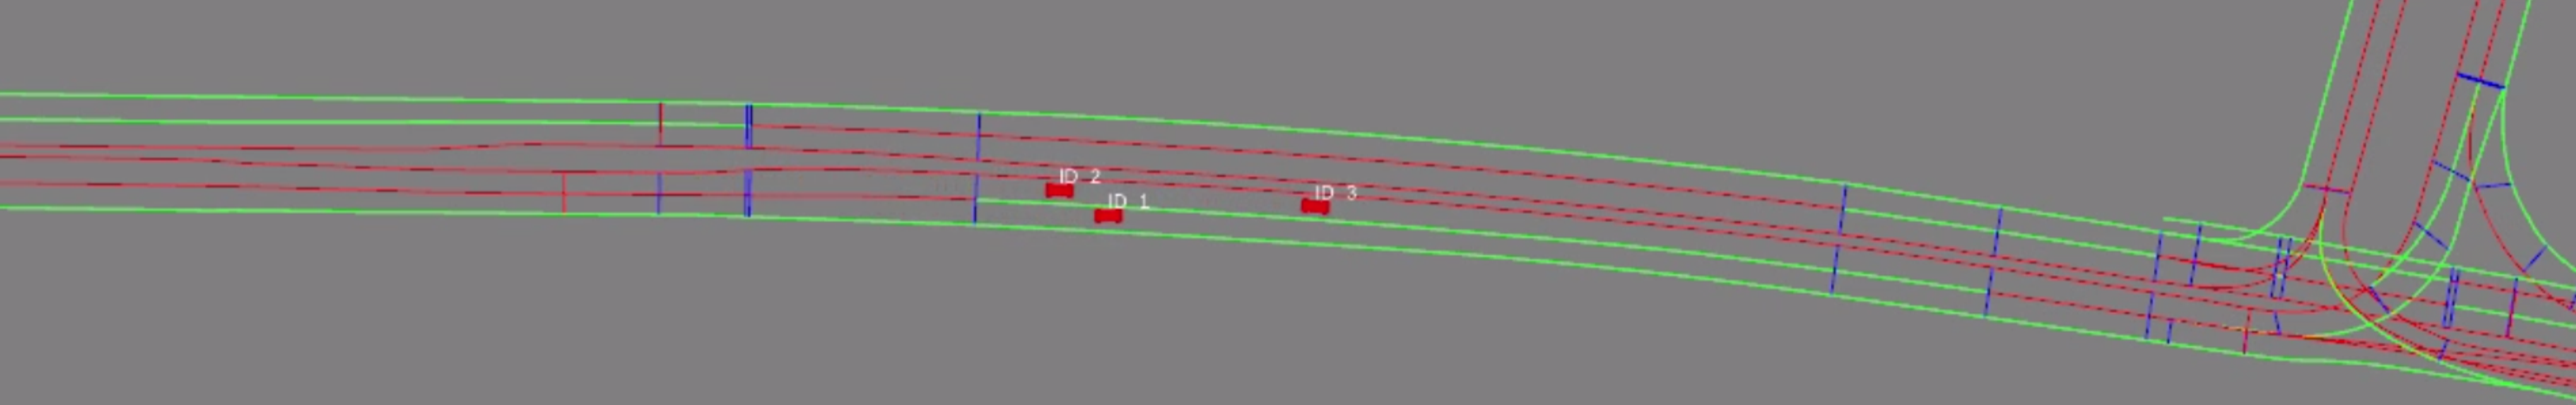
\includegraphics[width =  0.9 \textwidth]{egot_9.pdf}
    }
    \subfigure[t = 11s ]{
        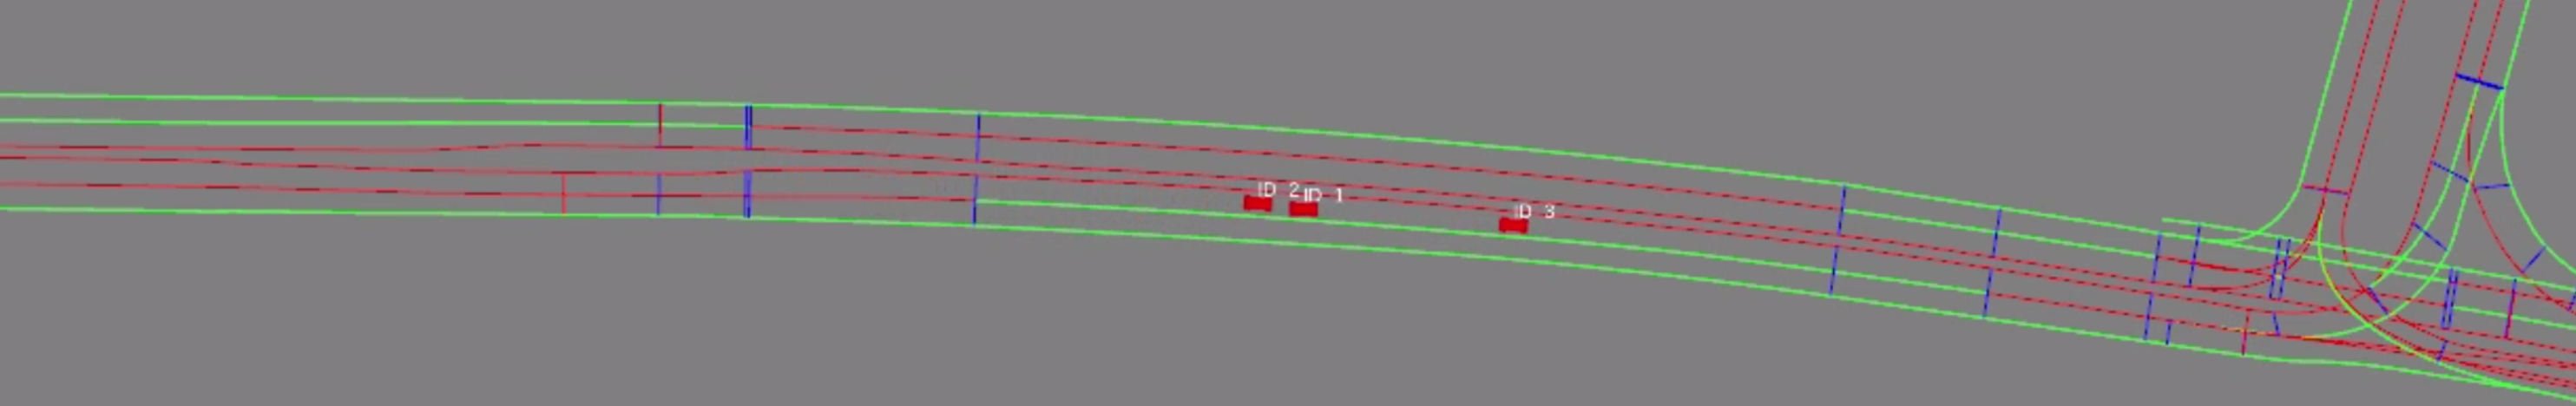
\includegraphics[width =  0.9 \textwidth]{egot_11.pdf}
    }
    \subfigure[t = 13s ]{
        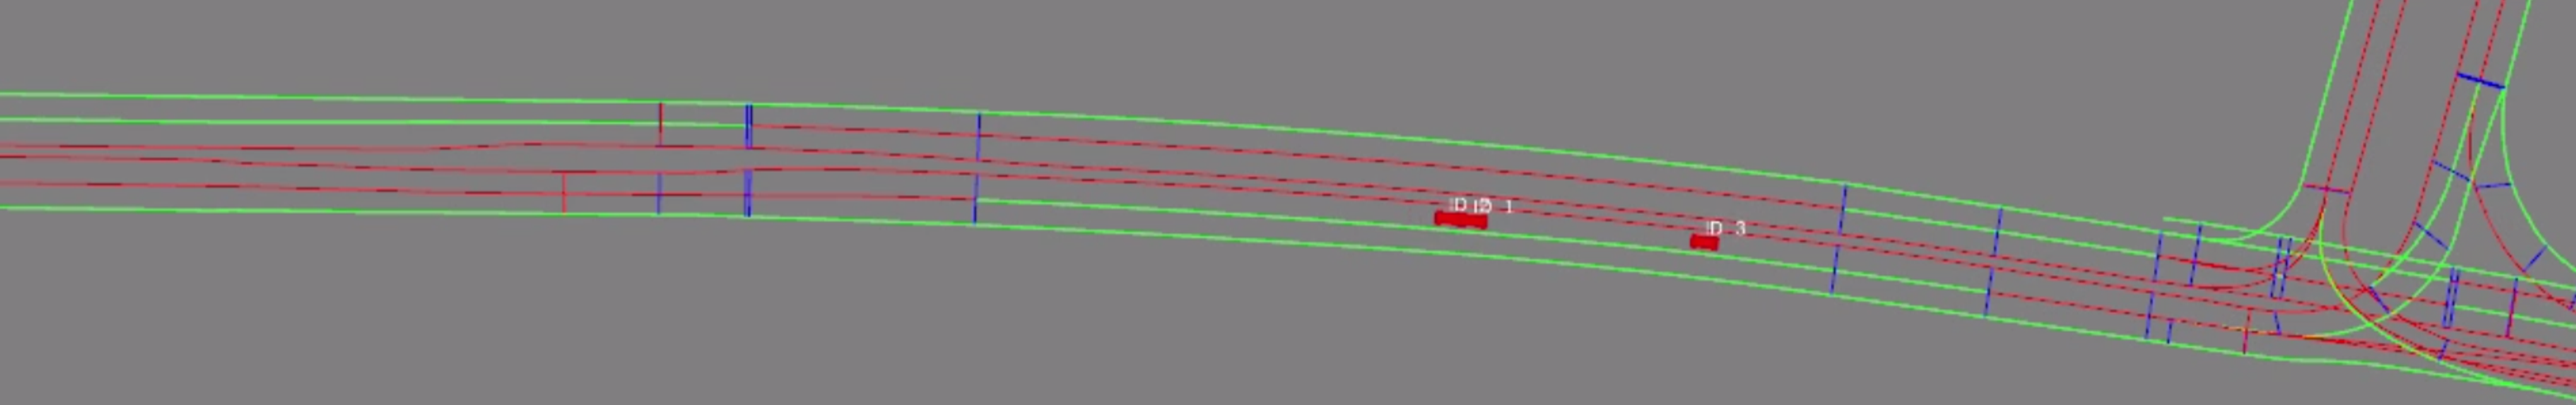
\includegraphics[width =  0.9 \textwidth]{egot_13.pdf}
    }
    \caption[Bildabfolge kooperativ]{Bildabfolge eines unkooperativen Fahrstreifenwechsels bei sek\"undlicher Neuplanung, bei dem das Ego"=Fahrzeug von einem kooperativen Verhalten ausgeht}
\end{figure}


\newpage
%--------------------------------------------------------------------------------
